\documentclass[12pt,letterpaper]{article}
\usepackage{graphicx} % Required for inserting images
\usepackage{parskip}
\graphicspath{{images/}}
\title{Applications of the First Law of Thermodynamics to flow processes}
\author{Medhaj Pawde \\ Github ID: 133995996 \\ ae22b004}


\date{June 2023}

\begin{document}
\maketitle
\section{\underline{Introduction}}
The general differential form of first law is stated as:
\begin{equation}
    \delta Q - \delta W = dE
\end{equation}
Here, \\ \(Q =\) Heat transfer \\
\(W =\) Work transfer \\
\(E =\) Energy associated with the system


This equation can only be used for processes involving closed systems.In the next section, We will generalise the modified form of the first law for control volume\cite{nag101engineering}
\section{\underline{First law for control volume}}
Consider an open system (fig:\ref{fig:myfigure}).We define the following quantites: 

$p_i,p_e$: Pressure (Pa) \\
$v_i,v_e$: Specific volume (m$^3$/kg)\\
$u_i,u_e$: Specific internal energy (J/kg) \\
$V_1$,$V_2$: \textnormal{Speed of the flow (m/s)} \\
$w_i,w_e$: Mass flow rate  
(kg/s) \\
$Z_i,Z_e$: Height from a fixed datum (m). \\
$\frac{\partial Q}{\partial \tau}$: Net rate of heat transfer (J/s). \\
$\frac{\partial W_x}{\partial \tau}$: Net rate of external work transfer (J/s).\\
$h_i,h_e$: specific enthalpy (J/kg).



Subscripts i and e refer to the inlet and exit sections.

\begin{figure}
    \centering
    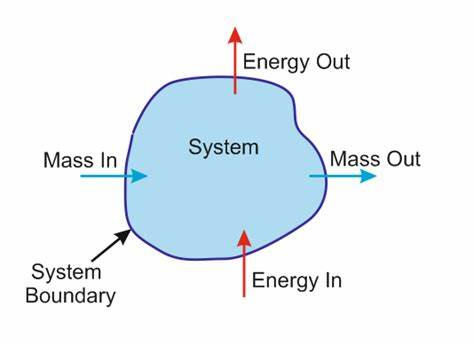
\includegraphics{FLoT.jpg}
    \caption{control volume.}
    \label{fig:myfigure}
\end{figure}



The first law for a flow process can be stated as \footnote{Here, we have ignored other contributions like nuclear energy, electronic energy etc.}:
\begin{equation}
    \frac{\partial Q}{\partial \tau} - \frac{\partial W_x}{\partial \tau} = \frac{dE}{d \tau} + \sum_e w_e[h_e + \frac{V_e^2}{2} + gZ_e] - \sum_i  w_i[h_i + \frac{V_i^2}{2} + gZ_i]
\end{equation}
\subsection{Special case}

For a steady flow process, there is no accumulation of mass or energy in the control volume.Therefore,
\[ \frac{dE}{d \tau} = 0\]
\[ \sum w_e = \sum w_i\]

\newpage
\bibliographystyle{plain}
\bibliography{PKN}

\end{document}
